\documentclass{article}

\PassOptionsToPackage{numbers,compress}{natbib}
\usepackage[eandd]{neurips_2026}

\usepackage[utf8]{inputenc}
\usepackage[T1]{fontenc}
\usepackage{hyperref}
\hypersetup{hidelinks}
\usepackage{url}
\usepackage{booktabs}
\usepackage{graphicx}
\usepackage{amsmath}
\usepackage{amssymb}
\usepackage{microtype}
\usepackage{multirow}
\usepackage{xspace}
\usepackage{xcolor}
\usepackage{enumitem}
\usepackage{nicefrac}

\newcommand{\bench}{TokenCapBench\xspace}
\newcommand{\success}{\mathrm{success}}
\newcommand{\budget}{B}
\newcommand{\ece}{\mathrm{ECE}}

\title{\bench: Forecasting Verified Success Under Token Caps}
\author{Anonymous Author(s)}

\begin{document}
\maketitle

\begin{abstract}
Language-model systems often commit inference resources before they know whether a run will succeed: a scheduler chooses which tasks to attempt, a router chooses a model, and a service sets a generated-token cap. Standard benchmarks usually report success at fixed inference settings, while token-use predictors estimate consumption rather than verified success. We introduce \textbf{TokenCapBench}, a verifier-backed benchmark for pre-execution success forecasting under imposed token caps. For each task, model, solver scaffold, verifier, and budget grid, a forecaster predicts the probability that a fresh capped solve will pass. The harness then executes independent solver calls under each cap, verifies every output, and evaluates both probability quality and strict no-overspend allocation. The release contains 1,542 core math and coding tasks with 33,008 verified capped outcomes across four models, plus scoped extensions for harder code generation, code editing, freshness, and timing diagnostics. Across tracks, verified success is strongly budget-dependent. Raw self-forecasts contain useful budget signal and improve 25\% fixed-budget scheduling over always using the maximum cap (150.2 versus 73.2 average core successes), but their probabilities remain miscalibrated: held-out empirical priors, histogram recalibration, and token-use proxy baselines are competitive or stronger for probability quality. By making success under a cap measurable, TokenCapBench provides a concrete target for building LLM systems that allocate inference budget with calibrated confidence.
\end{abstract}

\section{Introduction}

A deployed language-model system often has to commit inference resources before observing whether execution succeeds. A serving system may need to route a task to a cheaper or stronger model, cap a generation, defer an expensive request, or choose which tasks to attempt under a shared quota. Existing benchmarks mostly evaluate the downstream outcome: they choose a generation setting, run the model, and report whether the final answer passes. That is necessary for measuring capability, but it does not answer the earlier operational question: \emph{how likely is verified success under each available token cap?}

This question is distinct from response-length prediction. A short answer can pass, a long answer can fail, and extra tokens can help on one task while doing little on another. It is also distinct from ordinary confidence calibration, because the event is conditional on an imposed resource intervention. The relevant probability is not only $P(\success \mid x)$; it is $P(\success \mid x,m,s,\budget)$ for task $x$, model $m$, solver scaffold $s$, and generated-token cap $\budget$.

\bench makes this probability measurable. The forecasting call sees the task, solver conditions, verifier description, and budget grid, and is asked to output only probabilities. The harness then launches fresh solver contexts under each hard cap, hides the forecast from the solver, verifies every output, and scores both the probabilities and the budget choices induced by those probabilities. The central object is therefore a verified success curve under controlled token caps, not the token count of an unconstrained trajectory. Figure~\ref{fig:protocol} summarizes this separation between forecasting, budgeted solving, and verification.

This framing is deliberately narrower than a full agent benchmark. The first release uses controlled single-turn solve scaffolds and verifier-backed math and coding substrates. This constraint is a feature: it isolates the budget-conditioned forecasting problem before adding tool calls, retries, repository state, and production serving variability. The same protocol can later be embedded in agent controllers, but the present claims concern pre-execution forecasts under imposed generated-token budgets.

The paper makes four contributions.
\begin{enumerate}[leftmargin=*]
    \item We define \emph{pre-execution forecasting of verified success}: forecast first, intervene with hard generated-token caps, verify independently, and evaluate both calibration and allocation.
    \item We instantiate the protocol on verifier-backed math and coding tasks, including GSM8K, MATH/MATH-500, HumanEval+, MBPP+, BigCodeBench-Hard, CanItEdit, and LiveCodeBench freshness checks.
    \item We show that current models have partial budget awareness but weak raw calibration. Simple priors, lightweight recalibrators, and token-usage proxies often match or improve raw self-forecasts.
    \item We evaluate forecasts in the decision setting that motivates the benchmark: strict fixed-budget scheduling, where a policy must select task-budget pairs without overspending a global generated-token budget.
\end{enumerate}

\section{Related work}

\paragraph{Verifier-backed task benchmarks.}
GSM8K and MATH evaluate mathematical problem solving with answer checks \citep{cobbe2021training,hendrycks2021math}. HumanEval, MBPP, EvalPlus, BigCodeBench, CanItEdit, LiveCodeBench, and SWE-bench evaluate coding, editing, and repository-level capabilities with executable tests or official labels \citep{chen2021codex,austin2021program,liu2023evalplus,zhuo2024bigcodebench,cassano2023canitedit,jain2025livecodebench,jimenez2024swebench}. These benchmarks primarily measure final success under selected inference settings. \bench overlays a pre-execution forecasting problem on top of such substrates.

\paragraph{Calibration, self-knowledge, and selective prediction.}
Calibration metrics ask whether predicted probabilities match empirical frequencies \citep{brier1950verification,niculescu2005predicting,guo2017calibration}. Language-model work studies whether models know what they know and can express uncertainty reliably \citep{kadavath2022know,lin2022uncertainty}. Selective prediction studies when a model should answer at all \citep{geifman2017selective}. \bench changes the event being calibrated: the outcome is verified success under a specified generated-token cap, and the action space is budget selection rather than answer-or-abstain.

\paragraph{Token budgets and token consumption.}
Prior work studies response-length prediction for serving, token-budget-aware reasoning, adaptive token allocation, and inference-time scaling \citep{zheng2023response,han2025tale,li2025selfbudgeter,brown2024monkeys,snell2024scaling}. Recent agent-token work studies where agentic coding systems spend tokens and whether agents can predict their own unconstrained token usage \citep{bai2026tokenconsumption}. \bench is complementary: its budgets are imposed interventions, and its target is verifier-backed success under those interventions.


\begin{table}[t]
\centering
\small
\caption{\bench relative to neighboring evaluation problems. The central target is a pre-execution forecast of verifier-backed success under imposed generation budgets.}
\label{tab:related}
\resizebox{\linewidth}{!}{%
\begin{tabular}{lccccp{5.2cm}}
\toprule
Setting & Pre-exec. & Verified & Budget curve & Same task & What is missing for our target \\
\midrule
Verifier-backed task benchmarks & no & yes & no & yes & Measure solved/not-solved at fixed settings, not forecasts over budget interventions. \\
Confidence calibration / self-knowledge & yes & mixed & no & yes & Estimate correctness or uncertainty, but not success conditioned on explicit token caps. \\
Token-use or response-length prediction & yes & no & no & yes & Predict consumption of an unconstrained or served run, not verified success under a controlled cap. \\
Token-budgeting and test-time compute methods & sometimes & yes & sometimes & yes & Optimize or adapt spending, but do not benchmark pre-execution success-curve calibration. \\
\textbf{\bench} & \textbf{yes} & \textbf{yes} & \textbf{yes} & \textbf{yes} & \textbf{Forecasts and solve attempts are separated; each imposed budget is independently verified.} \\
\bottomrule
\end{tabular}%
}
\end{table}


Table~\ref{tab:related} summarizes the distinction: \bench evaluates calibrated success curves under imposed token caps, whereas neighboring settings usually fix a budget, predict token use, or adapt spending without separately benchmarking pre-execution success-curve calibration.

\section{Benchmark protocol}

Let $x$ be a task, $m$ a model, $s$ a solver scaffold, $V$ a verifier, and $\mathcal{B}=\{B_1,\ldots,B_K\}$ a grid of hard generated-token budgets. \bench evaluates $(x,m,s,V,\mathcal{B})$ in three phases.

\paragraph{Forecast.}
The model sees the task, solver conditions, verifier description, and budget grid. It is asked to output only probabilities, not a solution. The forecast is a structured map $\hat{p}(B)$ estimating the probability that a fresh solver run with generated-token cap $B$ will pass $V$.

\paragraph{Intervene.}
For each $B\in\mathcal{B}$, the harness launches a fresh solver context with cap $B$. The solver prompt excludes the forecast. This makes the budget an intervention and prevents the forecast from becoming a hidden control signal.

\paragraph{Verify and score.}
The verifier maps every budgeted output to a binary label $y(B)\in\{0,1\}$. The outcome matrix contains one task-budget row per capped solve attempt. Forecast quality is scored with Brier score and expected calibration error (ECE). Allocation quality is scored by the number of verified successes obtained when a policy selects task-budget pairs subject to a fixed global budget.

\begin{figure}[t]
\centering
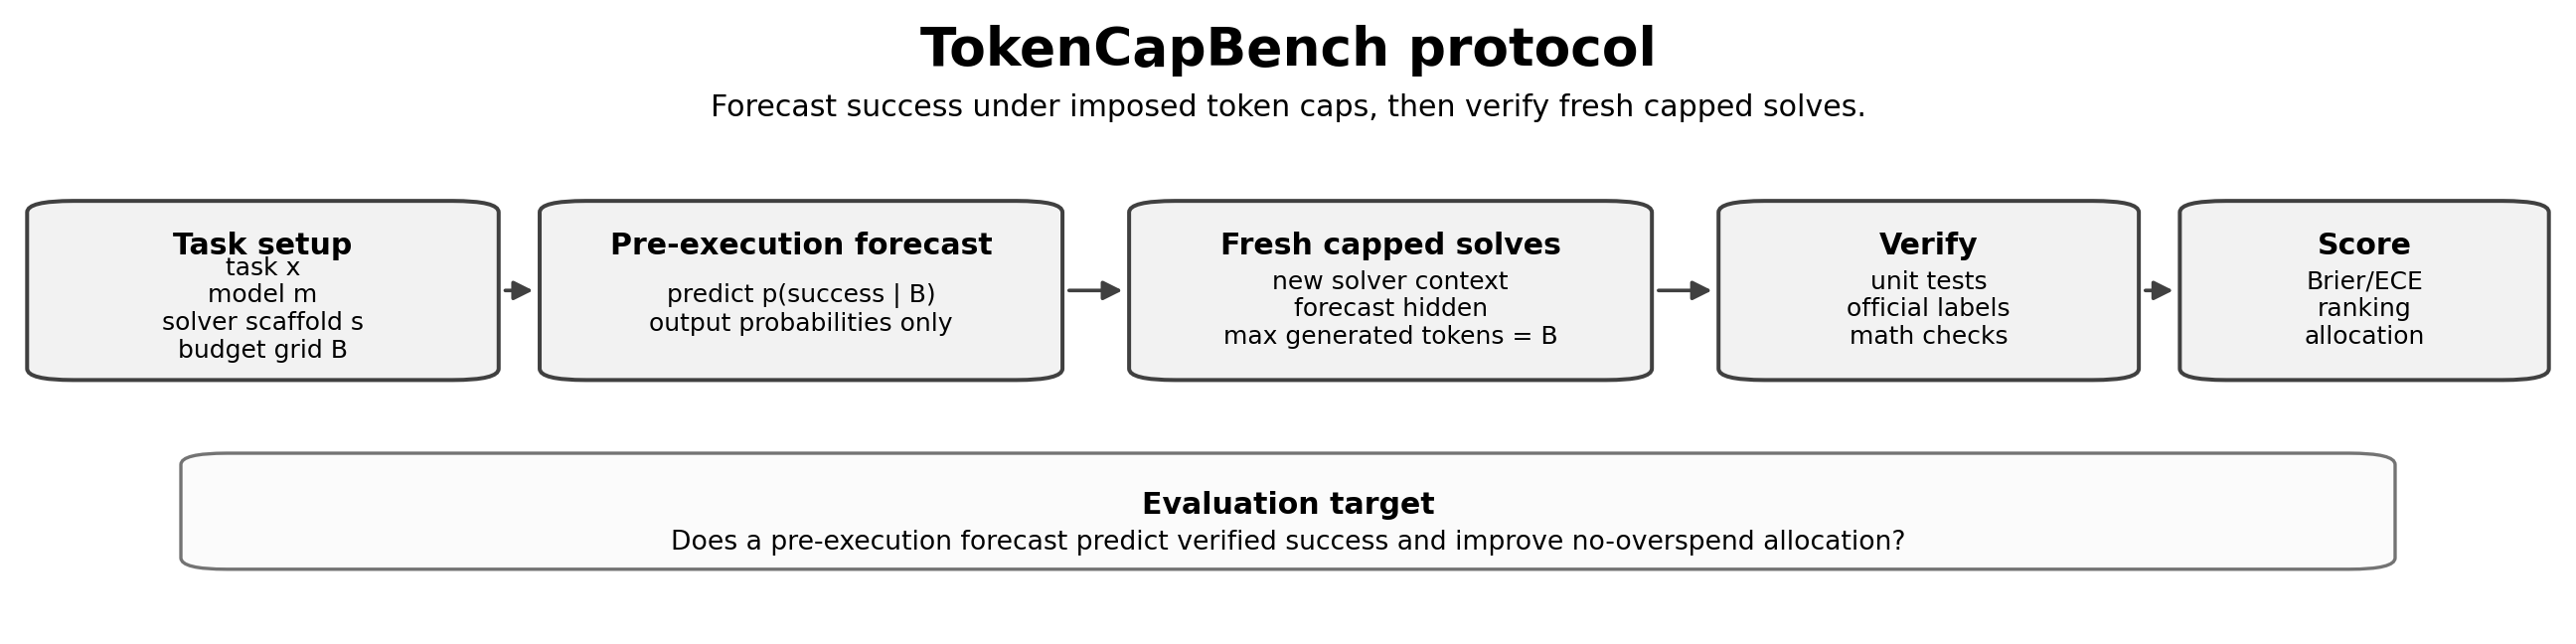
\includegraphics[width=\linewidth]{figures/figure1_protocol.png}
\caption{\bench protocol. A model forecasts a success-by-budget curve before solving. The benchmark then runs fresh capped solves, verifies each output independently, and evaluates both calibration and allocation.}
\label{fig:protocol}
\end{figure}

The first budget at which a task passes is the \emph{first-success budget}. Because success can be nonmonotone under stochastic generation and truncation, the benchmark retains the full success curve rather than forcing monotonicity. Allocation policies are evaluated on the observed matrix, not on smoothed curves.

\section{Evidence package and metrics}


\begin{table}[t]
\centering
\small
\caption{Evidence scope. Core claims use math and EvalPlus coding. Extension and diagnostic tracks test transfer and resource logging, but are scoped separately from the main claims.}
\label{tab:evidence}
\resizebox{\linewidth}{!}{%
\begin{tabular}{llrrrll}
\toprule
Role & Track & Tasks & Models & Outcome rows & Verifier / labels & Use in paper \\
\midrule
Core & GSM8K + MATH & 1000 & 4 & 20000 & numeric / symbolic & main calibration and allocation claims \\
Core & HumanEval+ + MBPP+ & 542 & 4 & 13008 & EvalPlus unit tests & main calibration and allocation claims \\
Extension & BigCodeBench-Hard & 148 & 5 & 4440 & package labels & hard practical coding extension \\
Extension & CanItEdit & 105 & 4 & 2100 & provided tests & code-editing bridge \\
Appendix & LiveCodeBench-300 & 300 & 2 & 3600 & official labels & freshness check \\
Diagnostic & timing/SLA subset & 100 & 2 & 3600 & same verifiers as core & resource logging only \\
\bottomrule
\end{tabular}%
}
\end{table}


Table~\ref{tab:evidence} summarizes the evidence package. The core evidence covers 1,000 math tasks and 542 EvalPlus coding tasks across four models, producing 33,008 verified capped solver outcomes. The row-level core outcome artifact is included in the external artifact store and has SHA-256 prefix \texttt{f2d07c91718e}. Extensions test whether the protocol transfers to harder practical coding (BigCodeBench-Hard), lightweight code editing (CanItEdit), and fresher coding tasks (LiveCodeBench-300). We use these extensions with explicit scope: BigCodeBench-Hard is the main hard-coding extension, CanItEdit is a provided-test editing bridge, and LiveCodeBench-300 is an appendix freshness check rather than a standalone main claim.

\paragraph{Forecast metrics.}
For each task-budget row $i$, Brier score is
\[
\frac{1}{n}\sum_{i=1}^{n}(\hat{p}_i-y_i)^2.
\]
ECE bins forecast probabilities and compares average confidence with empirical success frequency in each bin. We also report success at the maximum budget to separate solver capability from forecast quality. First-success-budget error, underbudgeting, overbudgeting, pairwise ranking accuracy, and regret diagnose how forecasts order tasks and budgets.

\paragraph{Operational allocation.}
The motivating decision is not just whether probabilities are calibrated; it is whether they support better budget choices. In strict fixed-budget scheduling, a policy selects at most one budget per task and must satisfy $\sum_i B_i \le C$ for a global generated-token budget $C$. Overspending is disallowed. We compare raw self-forecasts with empirical priors, recalibrators, token-usage proxies, random policies, max-budget policies, and oracle policies.

\paragraph{Resource accounting.}
The controlled intervention in the present paper is the generated-token cap. The harness also logs prompt tokens, completion tokens, total visible tokens, provider-exposed reasoning-token fields, finish reason, cap-hit/truncation flags, retry counts, and generation, verification, and end-to-end wall-clock timing when available. We treat timing as an appendix/SLA extension in this release because latency is noisier than token caps and requires repeated, controlled serving conditions to support main-paper claims.

\section{Results}

\subsection{Token budgets materially change verified success}

Figure~\ref{fig:core-success} shows nonflat success curves across generated-token caps. This supports the benchmark target: if success were nearly constant in budget, budget-conditioned forecasting would collapse to ordinary task success measurement. Instead, budget effects differ across task sources and models. Lines show canonical row-level success rates; bootstrap uncertainty summaries are included in the artifact reports.

\begin{figure}[t]
\centering
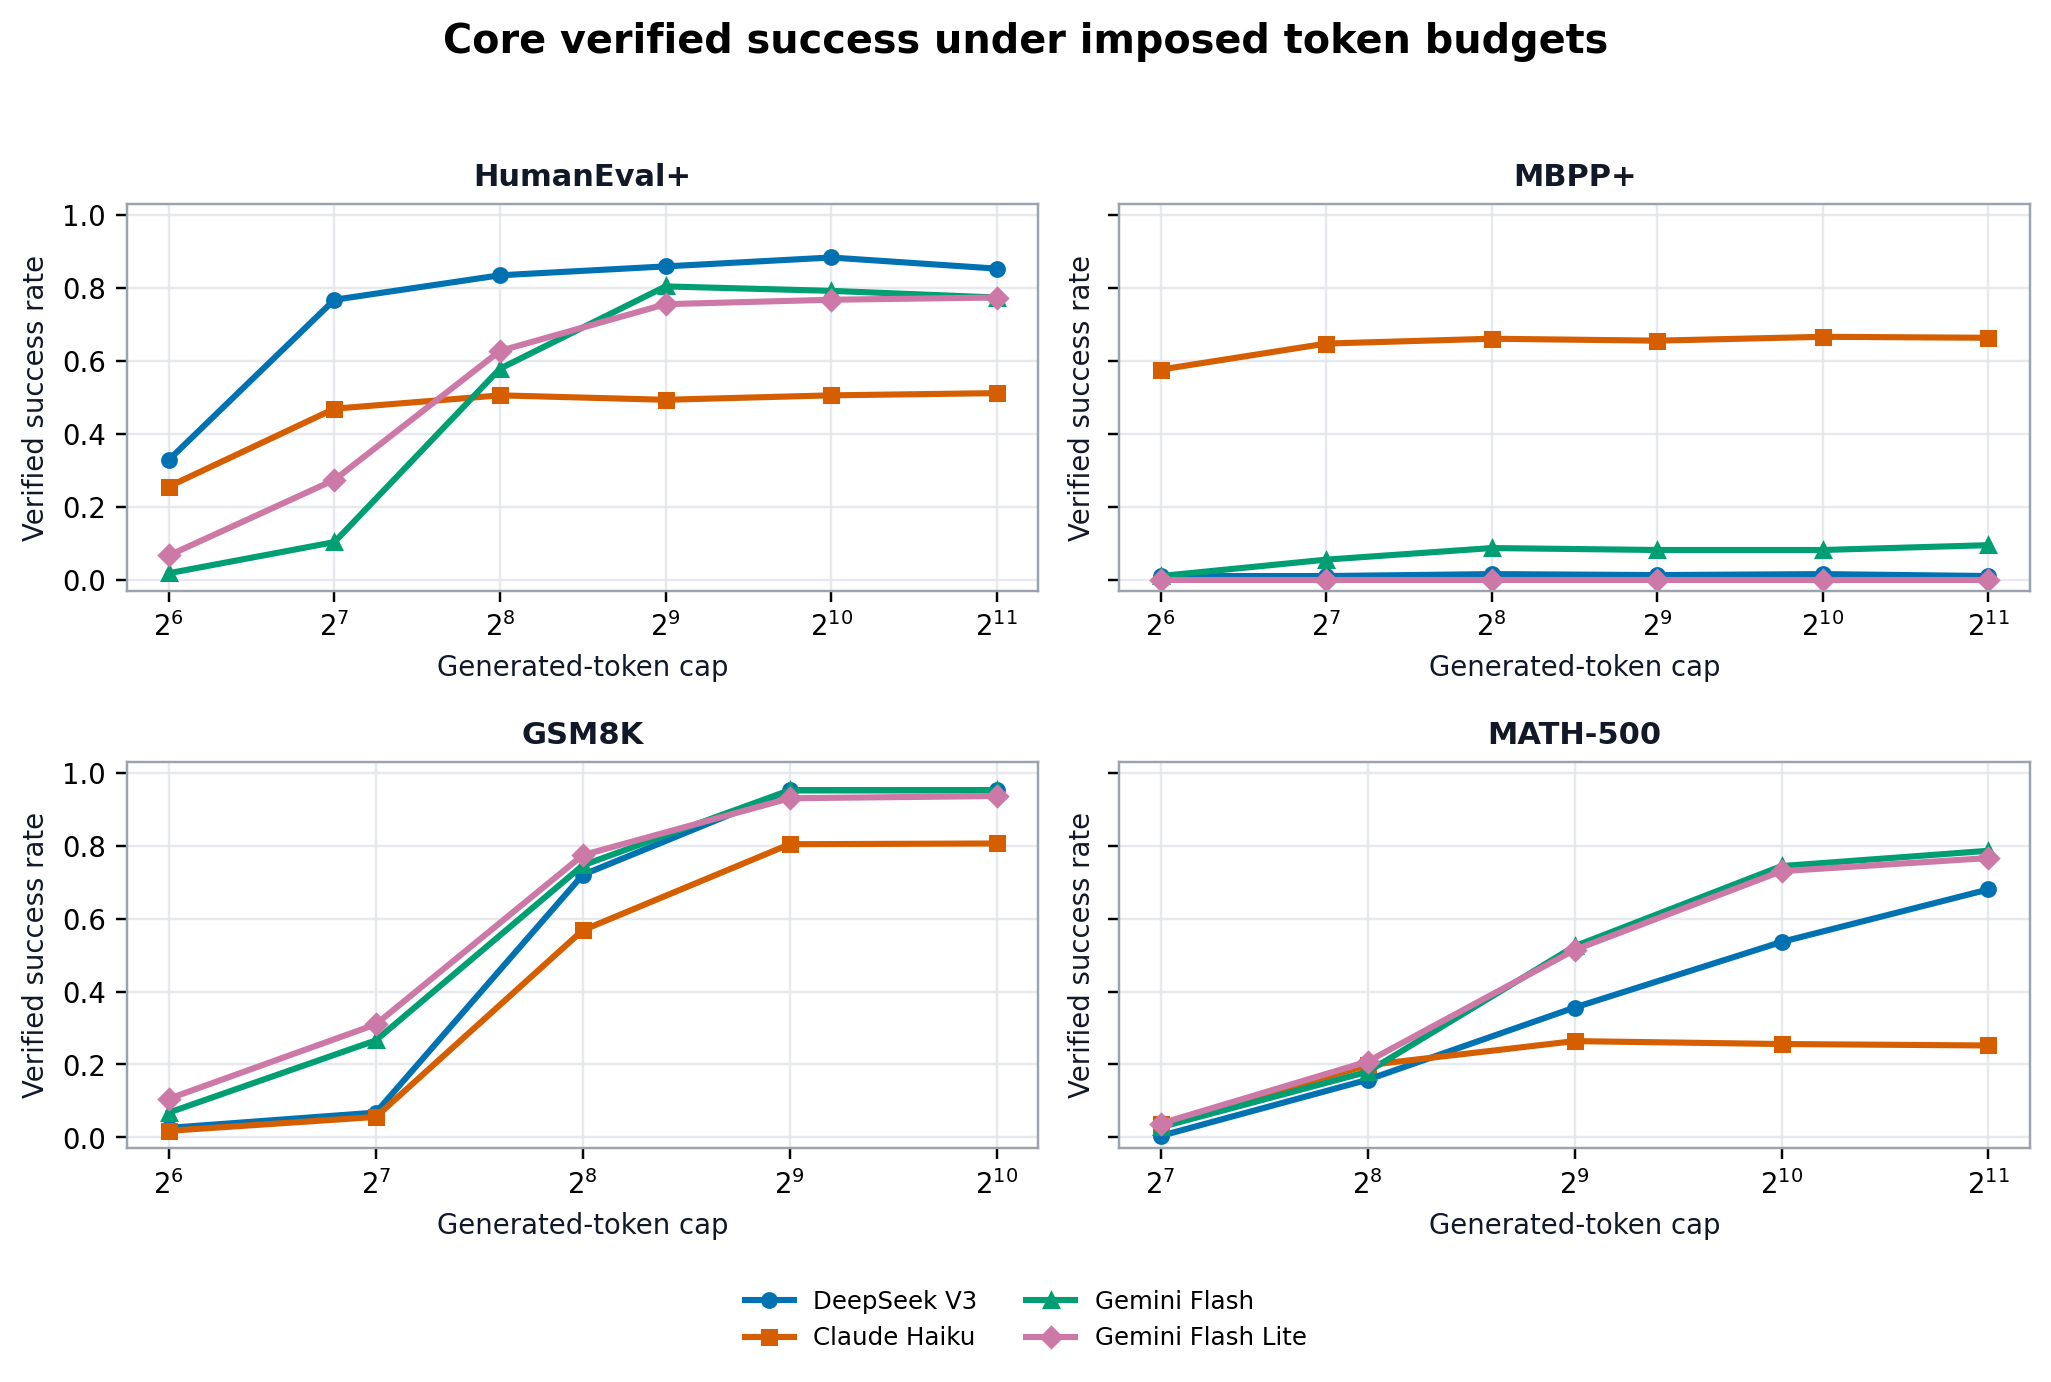
\includegraphics[width=\linewidth]{figures/paper_figure2_success_by_budget.png}
\caption{Verified success under imposed generated-token budgets on the core tracks. The math core is split into GSM8K and MATH-500 panels, and EvalPlus coding is split into HumanEval+ and MBPP+ panels. Confidence bands are omitted; lines show canonical row-level success rates.}
\label{fig:core-success}
\end{figure}

\begin{table}[t]
\centering
\small
\caption{Core-track summary regenerated from canonical row-level artifacts. Ranges are across models; baseline columns report held-out mean Brier across models. Lower Brier is better.}
\label{tab:core-summary}
\resizebox{\linewidth}{!}{%
\begin{tabular}{lccccccc}
\toprule
Suite & Models & Success@max & Raw Brier range & Rank acc. range & Raw Brier & Recal. Brier & Prior Brier \\
\midrule
HumanEval+ & 4 & 0.512-0.854 & 0.153-0.324 & 0.468-0.527 & 0.205 & 0.165 & 0.182 \\
MBPP+ & 4 & 0.000-0.664 & 0.299-0.460 & 0.276-0.476 & 0.256 & 0.191 & 0.222 \\
Math core & 4 & 0.529-0.869 & 0.127-0.255 & 0.564-0.798 & 0.184 & 0.151 & 0.174 \\
\bottomrule
\end{tabular}%
}
\end{table}


\subsection{Raw forecasts have signal, but calibration is not solved}

Table~\ref{tab:core-summary} shows partial budget awareness: forecast ranking and calibration vary meaningfully across suites and models, with MBPP+ exposing a particularly difficult near-all-failure regime for several models. This matters because a budget controller needs to rank both tasks and budgets before spending tokens. Figure~\ref{fig:baselines} makes the stronger conclusion clear: raw self-forecasts are not enough. Calibration-split priors and recalibrators often improve Brier score over raw forecasts. Models therefore expose budget-relevant information, but direct self-reports are not yet reliable probability estimates.

\begin{figure}[t]
\centering
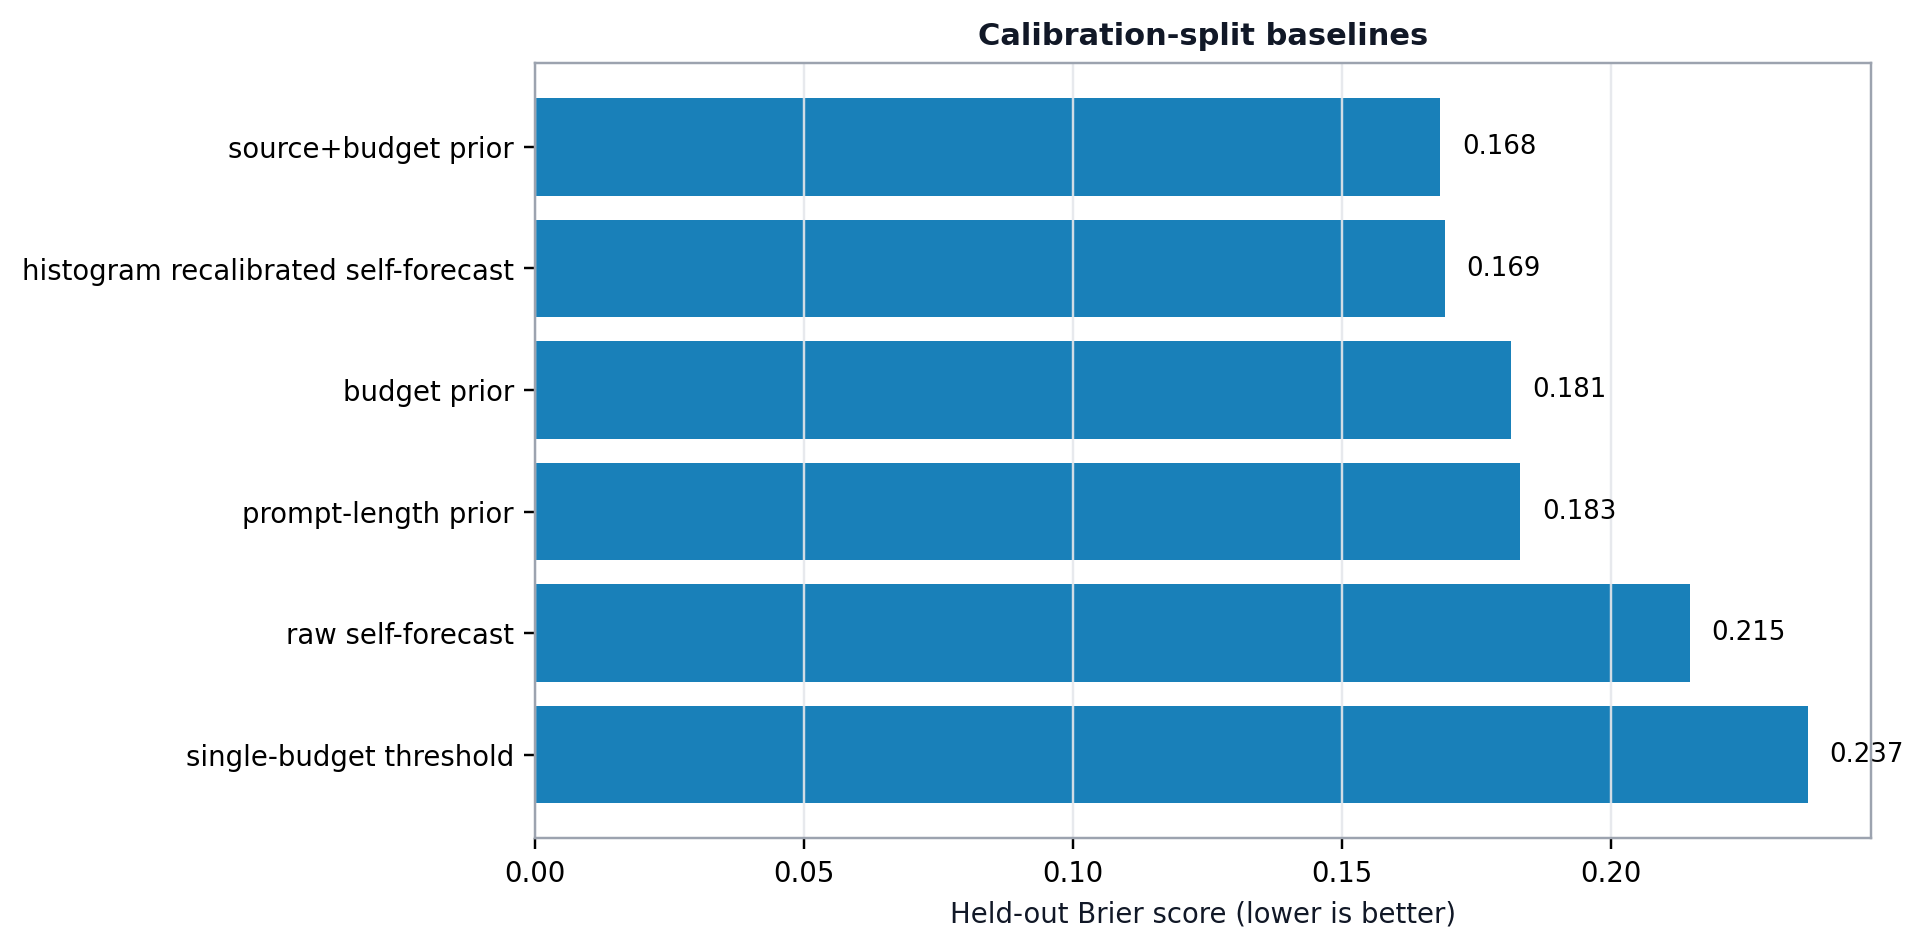
\includegraphics[width=0.92\linewidth]{figures/paper_figure5_calibration_split_baselines.png}
\caption{Calibration-split baseline comparison on held-out evaluation tasks. Raw self-forecasts contain signal, but empirical priors and recalibrated forecasts frequently match or improve on them. Lower Brier score is better.}
\label{fig:baselines}
\end{figure}

\subsection{Forecasts matter when they improve allocation}

Strict scheduling turns calibration into a decision problem. At a fixed global token budget, a scheduler must choose which task-budget pairs to run. Figure~\ref{fig:fixed-core} and Table~\ref{tab:scheduling} show this evaluation with zero overspend violations. On the core tracks at the 25 percent budget fraction, raw forecasts obtain 150.2 average verified successes, compared with 73.2 for always using the maximum cap and 137.2 for the best simple prior. This is the decision-facing comparison the benchmark is designed to support: a probability forecast is useful only if it improves verified utility under a real budget constraint.

\begin{figure}[t]
\centering
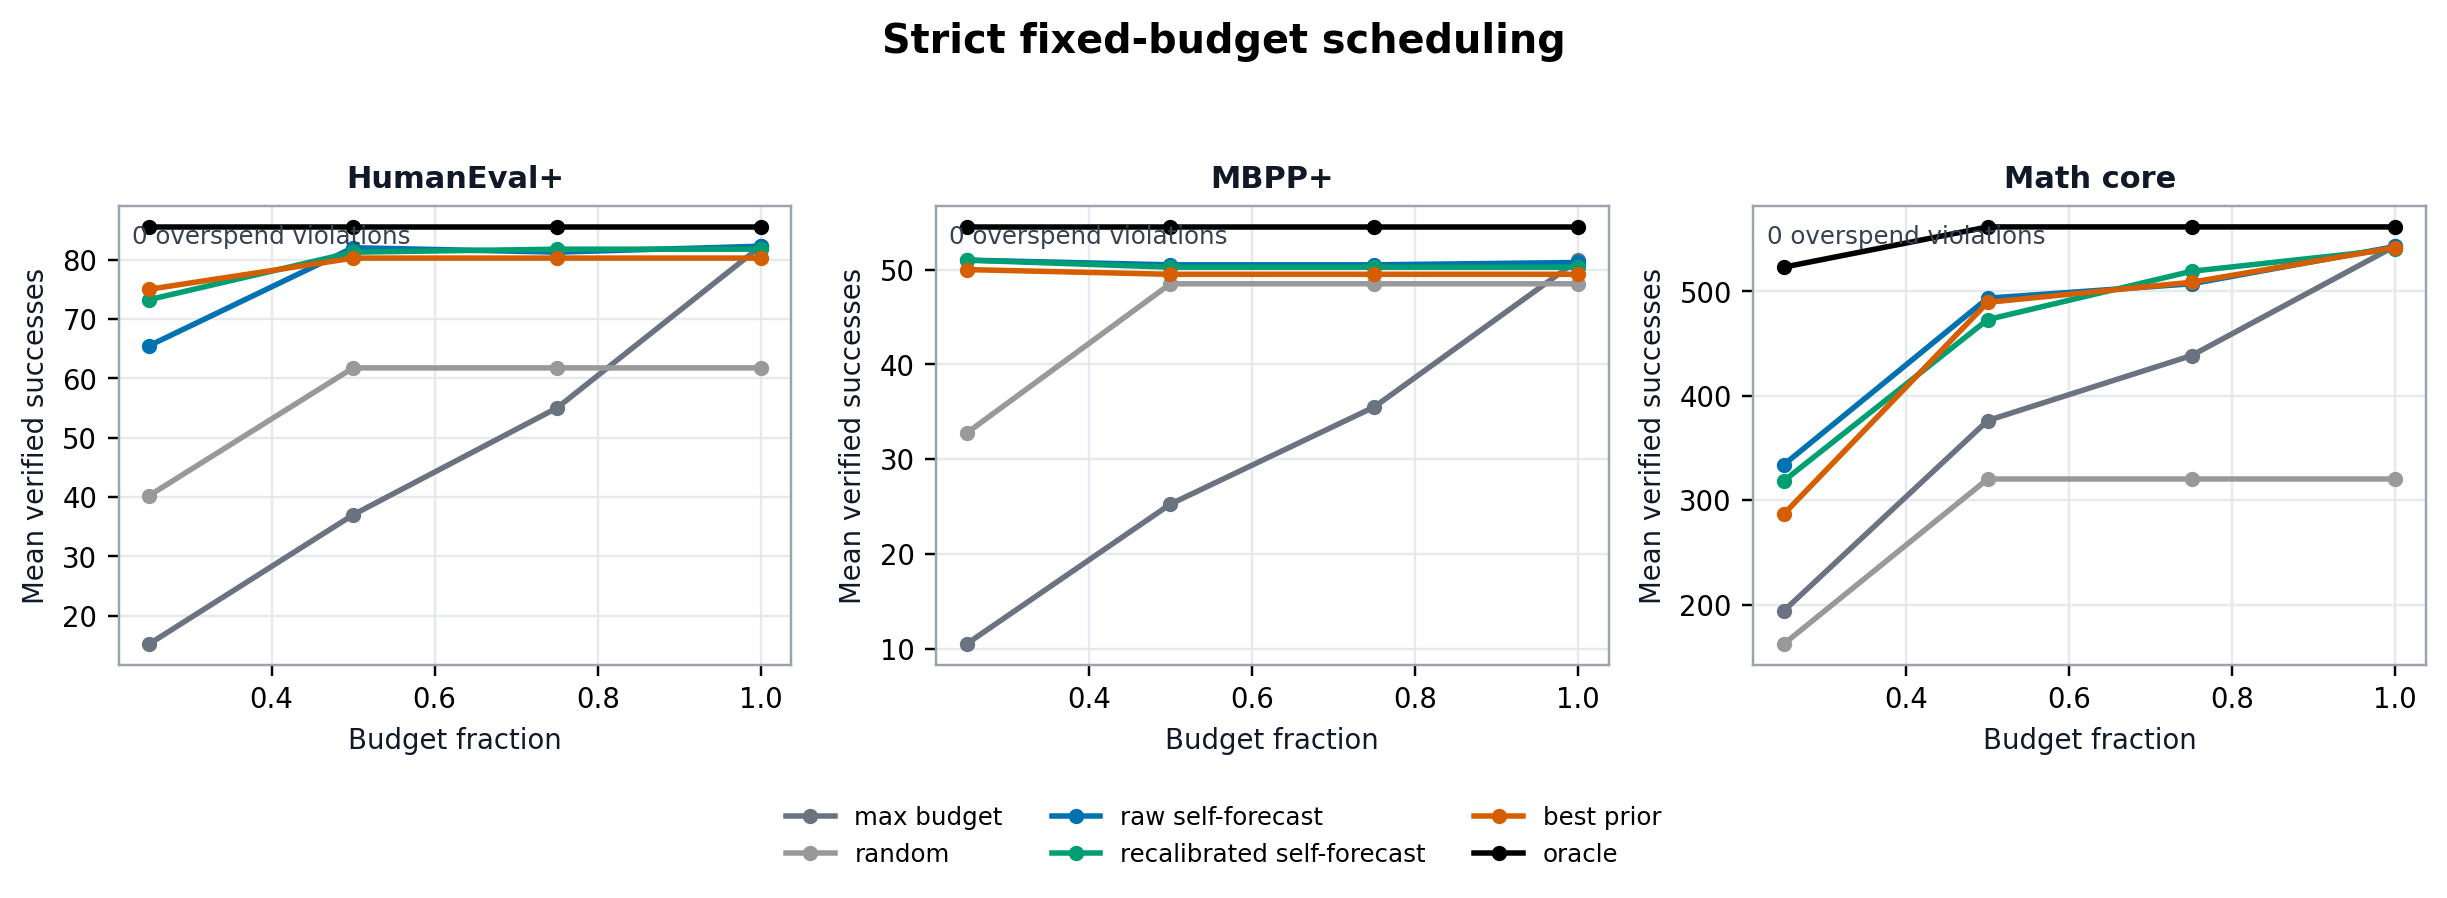
\includegraphics[width=\linewidth]{figures/paper_figure11_fixed_budget_scheduling.png}
\caption{Strict fixed-budget scheduling on the core tracks. Policies select task-budget pairs subject to the same global generated-token budget; the regenerated allocation table reports zero overspend violations.}
\label{fig:fixed-core}
\end{figure}


\begin{table}[t]
\centering
\small
\caption{Strict fixed-budget scheduling at the 25 percent core budget fraction. Rows are unweighted averages over core suite summaries and enforce zero overspend violations.}
\label{tab:scheduling}
\resizebox{\linewidth}{!}{%
\begin{tabular}{lrrrr}
\toprule
Policy & Avg. successes & Avg. regret to oracle & Avg. budget slack & Overspend viol. \\
\midrule
max budget & 73.2 & 147.8 & 31659 & 0 \\
random & 78.4 & 142.7 & 31147 & 0 \\
raw self-forecast & 150.2 & 70.9 & 31147 & 0 \\
recalibrated self-forecast & 147.6 & 73.5 & 47563 & 0 \\
best prior & 137.2 & 83.8 & 49600 & 0 \\
oracle & 221.1 & 0.0 & 80763 & 0 \\
\bottomrule
\end{tabular}%
}
\end{table}


\subsection{Hard coding and editing extensions are useful, but should be scoped carefully}

BigCodeBench-Hard extends the protocol to more practical Python generation with official package labels. CanItEdit provides a lightweight editing bridge with provided-test verification. Table~\ref{tab:extensions} and Figure~\ref{fig:ext-success} show that the same forecast-then-cap-then-verify protocol applies beyond HumanEval and MBPP. We do not present CanItEdit as a definitive hidden-test editing benchmark; its value here is to show that budget-conditioned forecasting naturally applies to edit-style prompts.

\input{tables/table_extensions}

\begin{figure}[t]
\centering
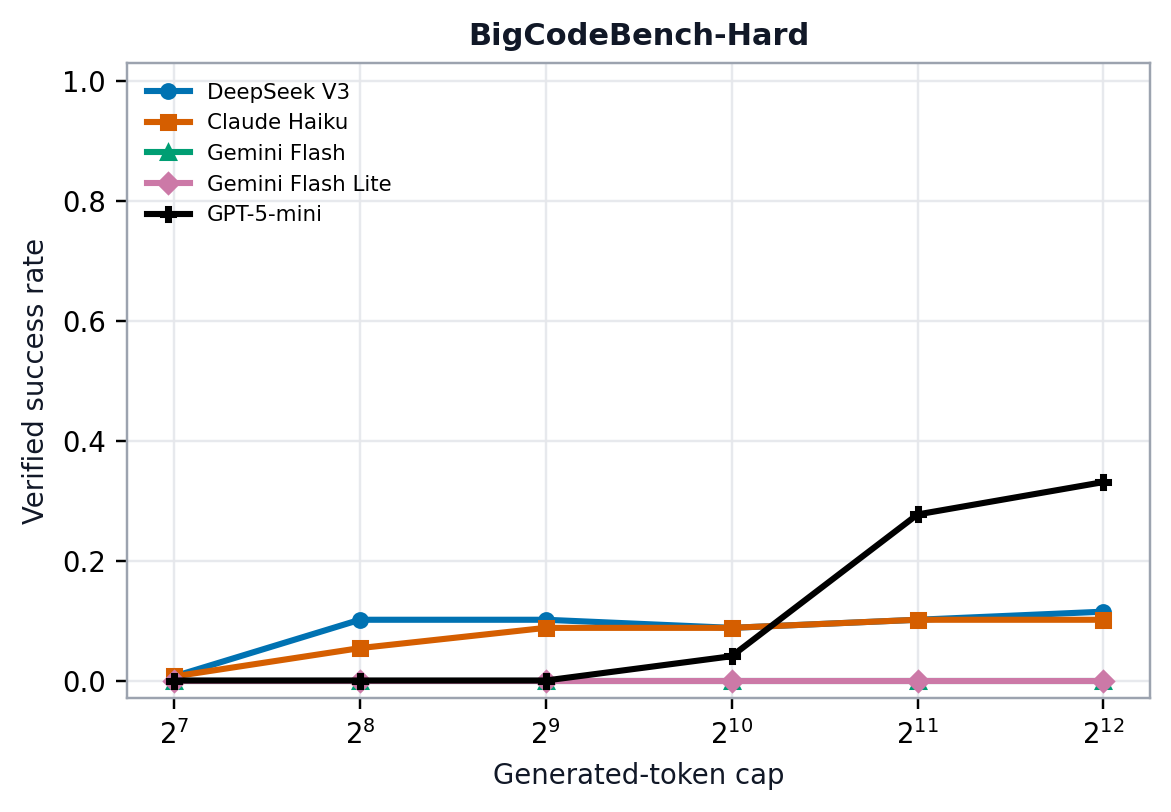
\includegraphics[width=0.49\linewidth]{figures/paper_figure11_bigcodebench_hard_success_by_budget.png}\hfill
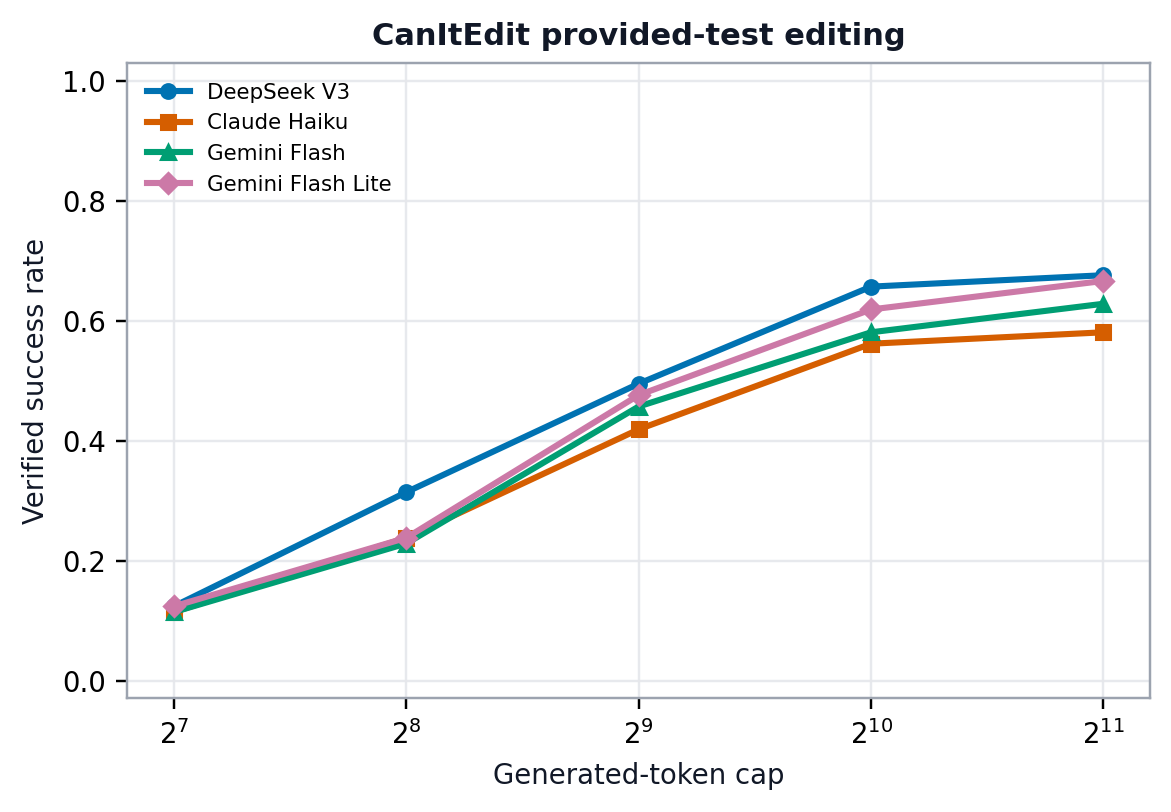
\includegraphics[width=0.49\linewidth]{figures/paper_figure12_canitedit_descriptive_success_by_budget.png}
\caption{Budget-success curves for practical coding extensions. Left: BigCodeBench-Hard with official package labels. Right: CanItEdit provided-test-only editing bridge.}
\label{fig:ext-success}
\end{figure}

\subsection{Token usage is a strong feature, not the benchmark target}

Token-usage forecasts and proxies can be highly informative. Table~\ref{tab:token-proxy} shows that token-proxy baselines can outperform raw success forecasts after being mapped to verified outcomes on calibration tasks. This does not make \bench redundant. Token-use prediction estimates resource consumption; \bench evaluates the verified utility available under imposed caps. A strong practical controller should use token features, task features, historical priors, and raw self-forecasts together, then be evaluated by calibrated success and allocation performance.


\begin{table}[t]
\centering
\small
\caption{Token-usage proxy comparison. Token-use predictions can be useful auxiliary features, but they are evaluated here only after being mapped to verified success under imposed budgets.}
\label{tab:token-proxy}
\resizebox{\linewidth}{!}{%
\begin{tabular}{lccccc}
\toprule
Suite & Usage coverage & Success-rank acc. & Token-proxy rank acc. & Raw success Brier & Token-proxy Brier \\
\midrule
BigCodeBench-Hard & 1.00 & 0.525 & 0.583 & 0.427 & 0.043 \\
HumanEval+ & 1.00 & 0.568 & 0.642 & 0.222 & 0.193 \\
MBPP+ & 1.00 & 0.421 & 0.573 & 0.401 & 0.075 \\
Math core & 1.00 & 0.704 & 0.729 & 0.170 & 0.165 \\
\bottomrule
\end{tabular}%
}
\end{table}


\section{Discussion}

\bench is strongest when framed as a benchmark for \emph{budgeted decision-making}, not as a generic token-consumption benchmark. The main empirical lesson is not that current models are hopeless or that raw self-forecasts are useless. The lesson is sharper: current models reveal partial information about budget-conditioned success, but simple baselines remain strong, and the practical value of a forecast only appears when it improves no-overspend allocation under a fixed budget.

The next version should add multi-resource success surfaces rather than replace the token-budget protocol. A deployment-oriented extension should evaluate success under service-level objectives: generated-token cap, total-token cap, wall-clock latency, retry budget, and provider-error budget. These should be reported as secondary resource metrics unless they are collected under repeated, controlled serving conditions. The target then becomes
\[
P(\success \mid x,m,s,\text{generated tokens},\text{total tokens},\text{latency},\text{retries}),
\]
with allocation evaluated on the same verified outcomes.

\section{Limitations}

The present release studies controlled single-turn solve scaffolds. It does not claim to evaluate full production agents, hidden reasoning compute, or Docker-heavy repository repair. CanItEdit uses provided tests, so we frame it as an editing bridge rather than a hidden-test editing result. LiveCodeBench-300 uses two models and remains a freshness check. Public benchmark contamination is possible on established datasets. Verifiers are imperfect: code labels inherit test-suite coverage, and math labels depend on answer extraction and symbolic/numeric matching.

Token counts are provider- and tokenizer-dependent. Generated-token caps do not measure all hidden inference compute, and wall-clock timing can vary with provider load, hardware, batching, and retry behavior. For that reason, timing is logged but not used for main claims in this release. These limitations define the first-release boundary and motivate the next benchmark version rather than invalidating the core protocol.

\section{Broader impact}

Budget-aware forecasting can make model use more transparent by exposing the expected success tradeoff of additional inference resources. It can also be misused if noisy forecasts are treated as guarantees or used to ration access without human oversight. We therefore frame \bench{} as an evaluation tool for calibrated decision support, not as an automatic policy for accepting, rejecting, or pricing user requests.

\section{Reproducibility and release status}

The repository includes task snapshots, prompts, forecast and outcome schemas, metric code, compact tables and figures, run manifests, a benchmark card, data provenance notes, a reproduction guide, Croissant metadata, and validation scripts. Table~\ref{tab:validation} gives the current validation summary for the frozen paper artifacts. The artifact is packaged as a local release archive for anonymous supplementary submission; a stable hosted URL can be added in the submission form when assigned.

\input{tables/table_validation}

\section{Conclusion}

\bench asks a concrete question that ordinary task benchmarks and token-consumption predictors do not answer: before execution, how likely is verified success under each imposed token cap? The forecast-then-intervene protocol separates self-assessment from solving, imposes hard generated-token caps, verifies every outcome, and evaluates both calibration and allocation. The current evidence shows that budget-conditioned success is real, raw self-forecasts are informative but miscalibrated, and strict fixed-budget scheduling exposes the operational effect of those forecasts. This creates a clear target for future forecasters and controllers: choose budgets before execution with calibrated expectations of verifier-backed success.

\clearpage
\bibliographystyle{plainnat}
\bibliography{references}

\clearpage
\appendix
\section{Additional implementation details}
\label{app:implementation}
The benchmark logs generated-token budget, finish reason, cap-hit/truncation flag, prompt tokens, completion tokens, total visible tokens, provider-exposed reasoning-token fields, retry count, generation wall time, verification wall time, and end-to-end wall time. The main results use generated-token caps because they are the controlled intervention shared across the current tracks. The logged timing, retry, and total-token fields are intended for SLA-style extensions and resource-accounting diagnostics.

Recommended secondary metrics for the artifact are log score after probability clipping, bootstrap confidence intervals over tasks, cap-hit rate, retry rate, p50/p95 generation latency, p50/p95 verification latency, end-to-end latency, and throughput in tokens per second. These metrics should be reported in the appendix or artifact card unless the experiment uses repeated measurements on stable serving infrastructure.

\section{Checklist}
\section*{NeurIPS Paper Checklist}

\begin{enumerate}

\item {\bf Claims}
    \item[] Question: Do the main claims made in the abstract and introduction accurately reflect the paper's contributions and scope?
    \item[] Answer: \answerYes{}.
    \item[] Justification: The abstract and introduction state the benchmark protocol, the verifier-backed evidence scope, and the limits of raw self-forecast calibration.

\item {\bf Limitations}
    \item[] Question: Does the paper discuss the limitations of the work performed by the authors?
    \item[] Answer: \answerYes{}.
    \item[] Justification: The Limitations section covers public benchmark contamination, verifier coverage, hidden reasoning compute, provider/tokenizer cap dependence, and timing variability.

\item {\bf Theory assumptions and proofs}
    \item[] Question: For each theoretical result, does the paper provide the full set of assumptions and a complete proof?
    \item[] Answer: \answerNA{}.
    \item[] Justification: The paper introduces and evaluates a benchmark protocol; it does not claim new theoretical results.

\item {\bf Experimental result reproducibility}
    \item[] Question: Does the paper disclose the information needed to reproduce the main experimental results?
    \item[] Answer: \answerYes{}.
    \item[] Justification: The repository includes task snapshots, prompts, schemas, canonical row-level forecast/outcome artifacts, metric code, and regeneration scripts.

\item {\bf Open access to data and code}
    \item[] Question: Does the paper provide open access to the data and code, with sufficient instructions to reproduce the main experimental results?
    \item[] Answer: \answerYes{}.
    \item[] Justification: The release archive contains the code, compact tables and figures, external artifact manifest, Croissant metadata, and canonical row-level artifacts. Anonymous hosted URL assignment remains author-owned.

\item {\bf Experimental setting/details}
    \item[] Question: Does the paper specify the experimental setting details necessary to understand the results?
    \item[] Answer: \answerYes{}.
    \item[] Justification: The protocol, budget grids, forecast/solve separation, verifier-backed task sources, calibration split, and strict allocation setting are described in the paper and artifact docs.

\item {\bf Experiment statistical significance}
    \item[] Question: Does the paper report error bars or other appropriate information about statistical significance?
    \item[] Answer: \answerYes{}.
    \item[] Justification: Tables report bootstrap intervals where available. The regenerated Figure 2 caption explicitly states that confidence bands are omitted for direct row-level success curves.

\item {\bf Experiments compute resources}
    \item[] Question: Does the paper provide sufficient information on compute resources needed to reproduce the experiments?
    \item[] Answer: \answerYes{}.
    \item[] Justification: The artifact logs generated-token caps, token usage fields, retry counts, wall-clock timing, and cost/runtime summaries; timing is scoped as diagnostic rather than a provider benchmark.

\item {\bf Code of ethics}
    \item[] Question: Does the research conform with the NeurIPS Code of Ethics?
    \item[] Answer: \answerYes{}.
    \item[] Justification: The work evaluates benchmark artifacts and model outputs on public/verifier-backed tasks without human subjects or sensitive personal data collection.

\item {\bf Broader impacts}
    \item[] Question: Does the paper discuss positive and negative societal impacts?
    \item[] Answer: \answerYes{}.
    \item[] Justification: The Broader impact section discusses transparent budget-aware decision support and the risk of treating noisy forecasts as guarantees.

\item {\bf Safeguards}
    \item[] Question: Does the paper describe safeguards for responsible release of high-risk data or models?
    \item[] Answer: \answerNA{}.
    \item[] Justification: The paper releases benchmark artifacts and code, not a model or high-risk scraped dataset; release metadata and secret-scrub checks are included.

\item {\bf Licenses for existing assets}
    \item[] Question: Are existing assets properly credited and are license and terms of use mentioned?
    \item[] Answer: \answerYes{}.
    \item[] Justification: The paper cites the underlying benchmark sources and the repository includes license, citation, benchmark card, data provenance, Croissant metadata, and release manifests.

\item {\bf New assets}
    \item[] Question: Are new assets introduced in the paper documented and provided alongside the assets?
    \item[] Answer: \answerYes{}.
    \item[] Justification: TokenCapBench artifacts are documented through the README, benchmark card, data provenance note, reproduction guide, Croissant metadata, and release manifests.

\item {\bf Crowdsourcing and research with human subjects}
    \item[] Question: For crowdsourcing experiments and research with human subjects, does the paper include the required participant information?
    \item[] Answer: \answerNA{}.
    \item[] Justification: The work does not involve crowdsourcing experiments or human subjects research.

\item {\bf Institutional review board approvals or equivalent for research with human subjects}
    \item[] Question: Does the paper describe risks, disclosures, and approvals for human subjects research?
    \item[] Answer: \answerNA{}.
    \item[] Justification: The work does not involve human subjects research.

\item {\bf Declaration of LLM usage}
    \item[] Question: Does the paper describe LLM usage if it is an important or non-standard component of the research?
    \item[] Answer: \answerYes{}.
    \item[] Justification: LLMs are the forecast and solver subjects of the benchmark, and the protocol describes their role and separation.

\end{enumerate}


\end{document}
